This Appendix contains 9 ranking plots from the \wh{} STXS fit.

\begin{figure}[htp]
    \centering
    \subfloat[Ranking: $0 < \ptv{} < 75$~GeV.]{
        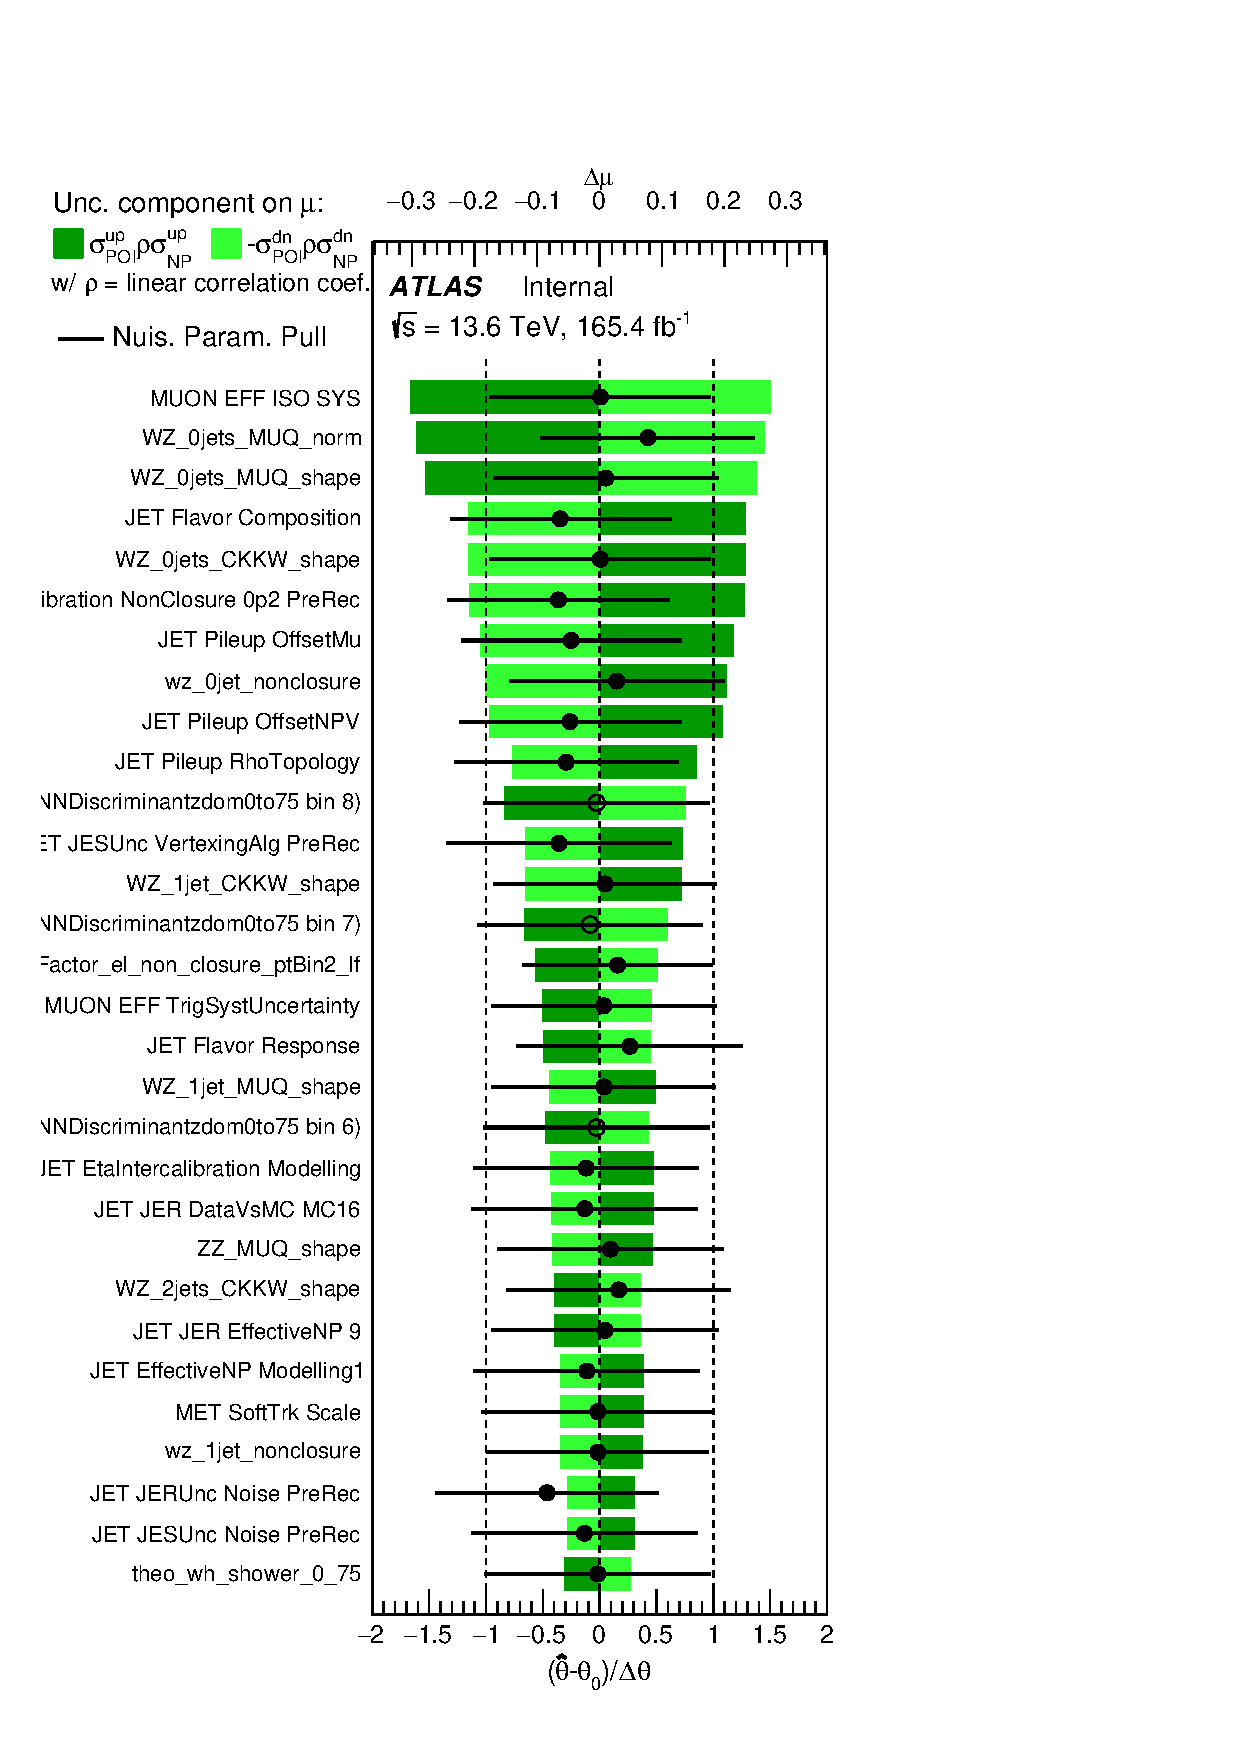
\includegraphics[width=0.3\linewidth]{figures/appendix/wh_stxs_results/rankings/Ranking_mu_WH_0_75_Breakdown_zdom_stxs.pdf}
    }
    \subfloat[Ranking: $75 < \ptv{} < 150$~GeV.]{
        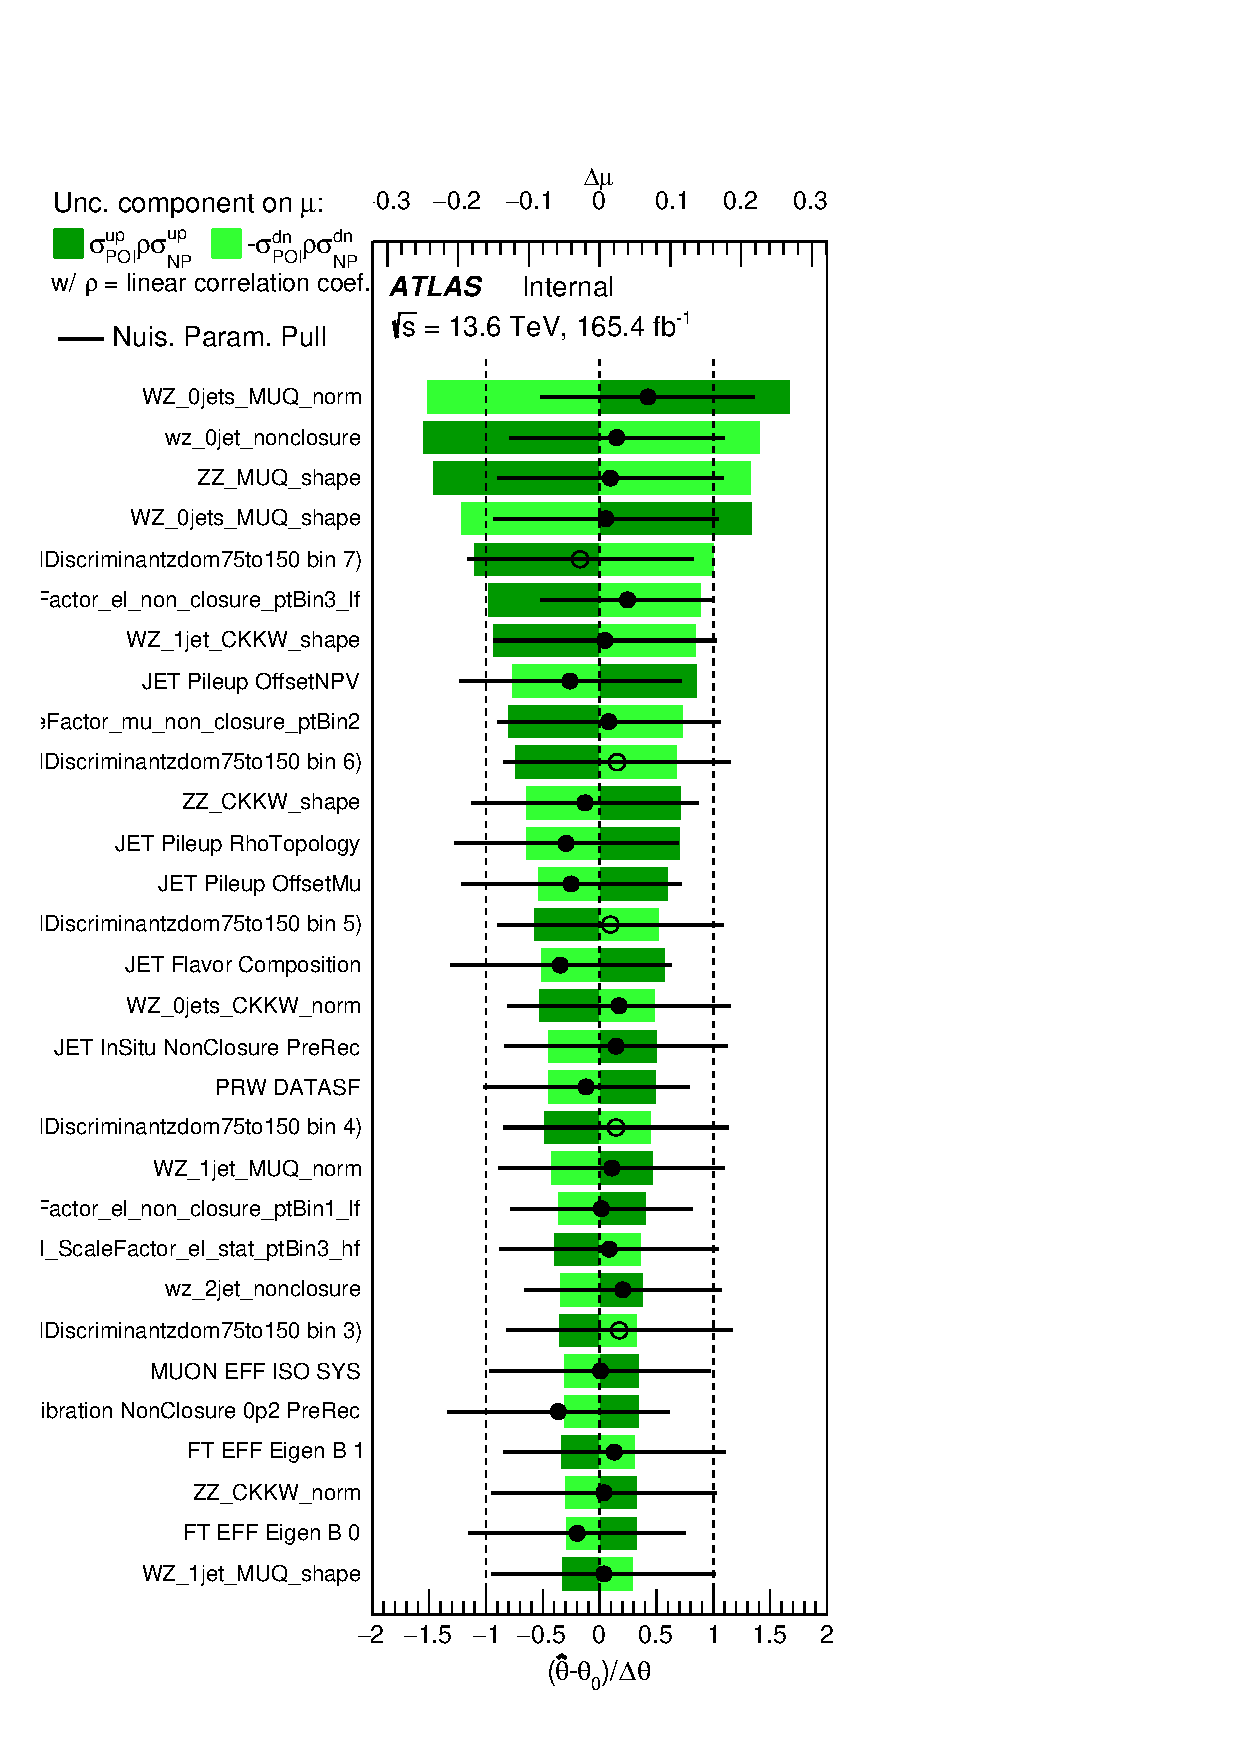
\includegraphics[width=0.3\linewidth]{figures/appendix/wh_stxs_results/rankings/Ranking_mu_WH_75_150_Breakdown_zdom_stxs.pdf}
    }
    \subfloat[Ranking: $\ptv{} > 150$~GeV.]{
        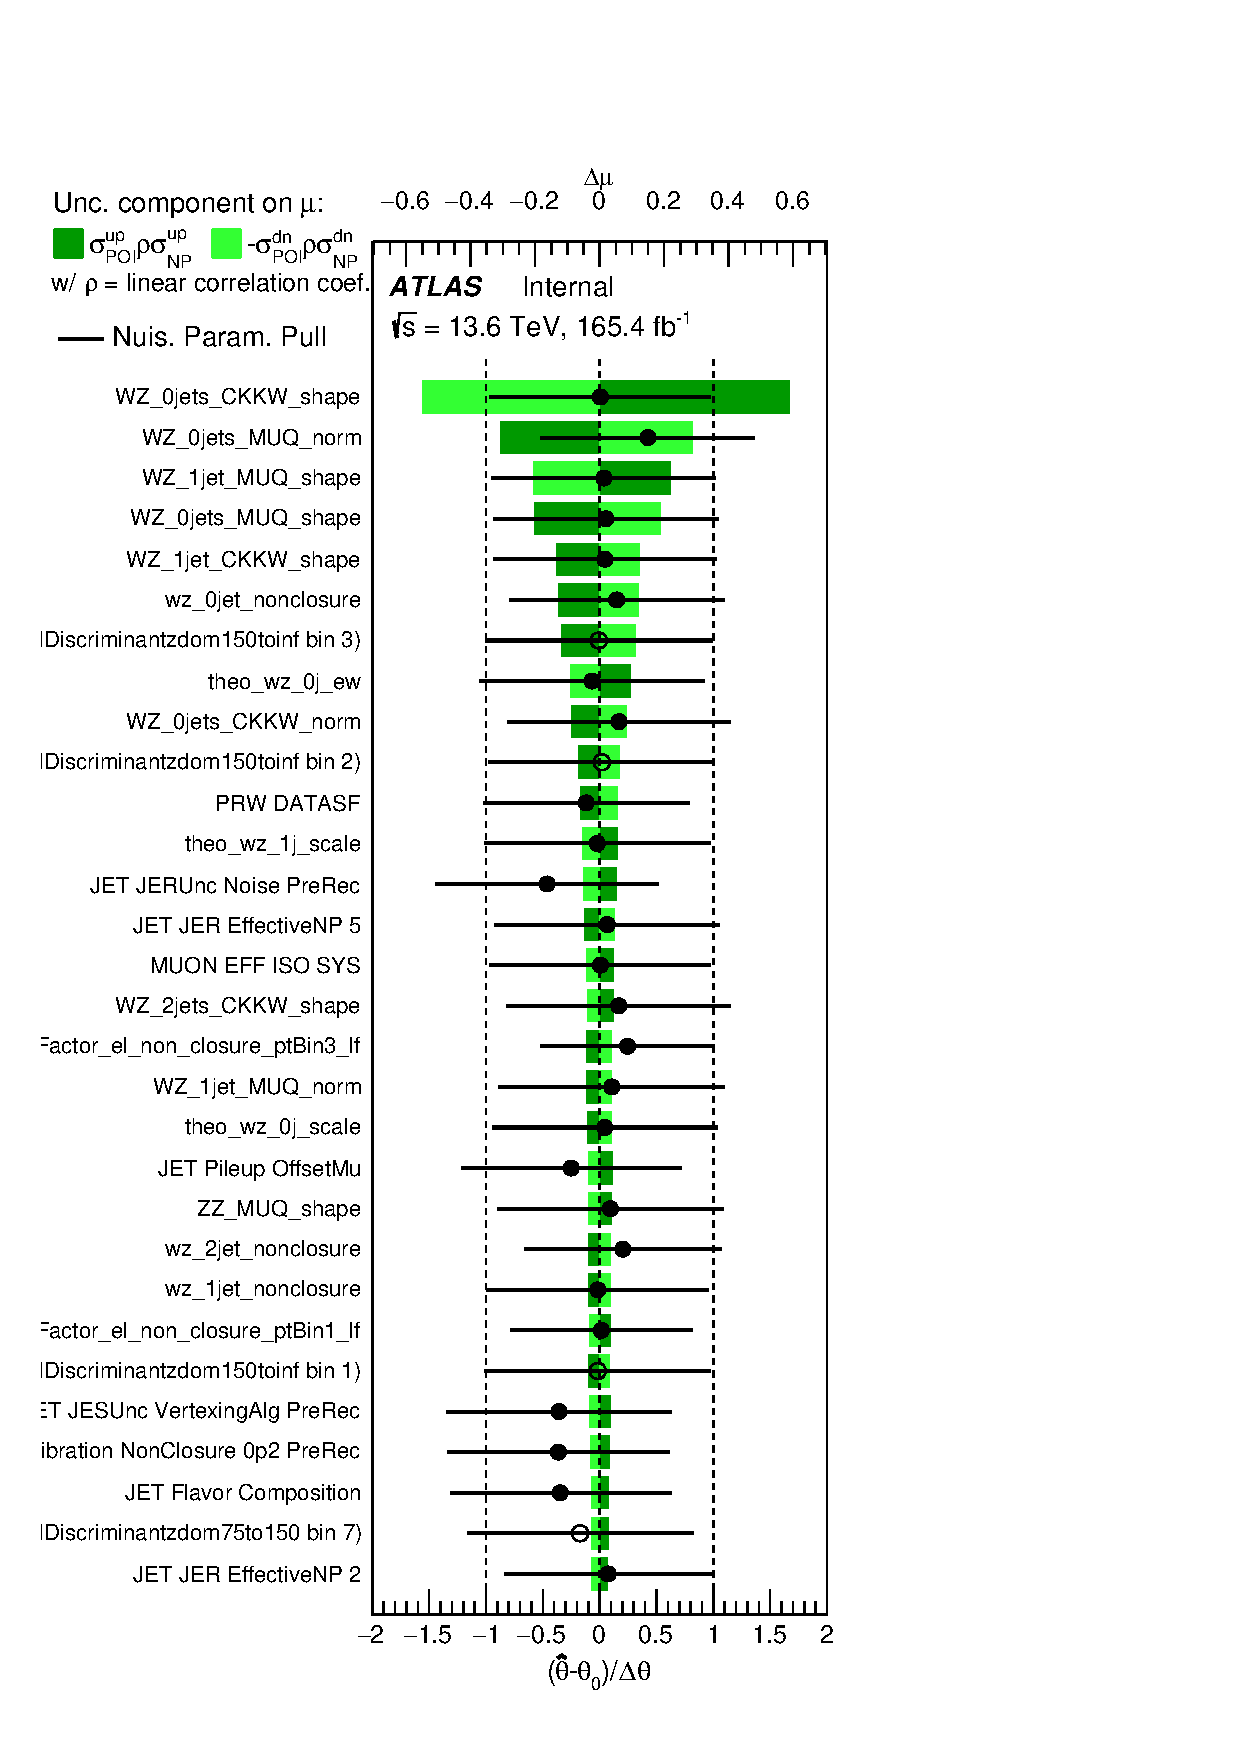
\includegraphics[width=0.3\linewidth]{figures/appendix/wh_stxs_results/rankings/Ranking_mu_WH_150_inf_Breakdown_zdom_stxs.pdf}
    }
    \caption{Systematic ranking plots for the \zdom{} \wh{} STXS signal regions: (a) $0 < \ptv{} < 75$~GeV, (b) $75 < \ptv{} < 150$~GeV, and (c) $\ptv{} > 150$~GeV.}\label{fig:wh_stxs_ranking_plots_zdom}
\end{figure}

\begin{figure}[htp]
    \centering
    \subfloat[Ranking: $0 < \ptv{} < 75$~GeV.]{
        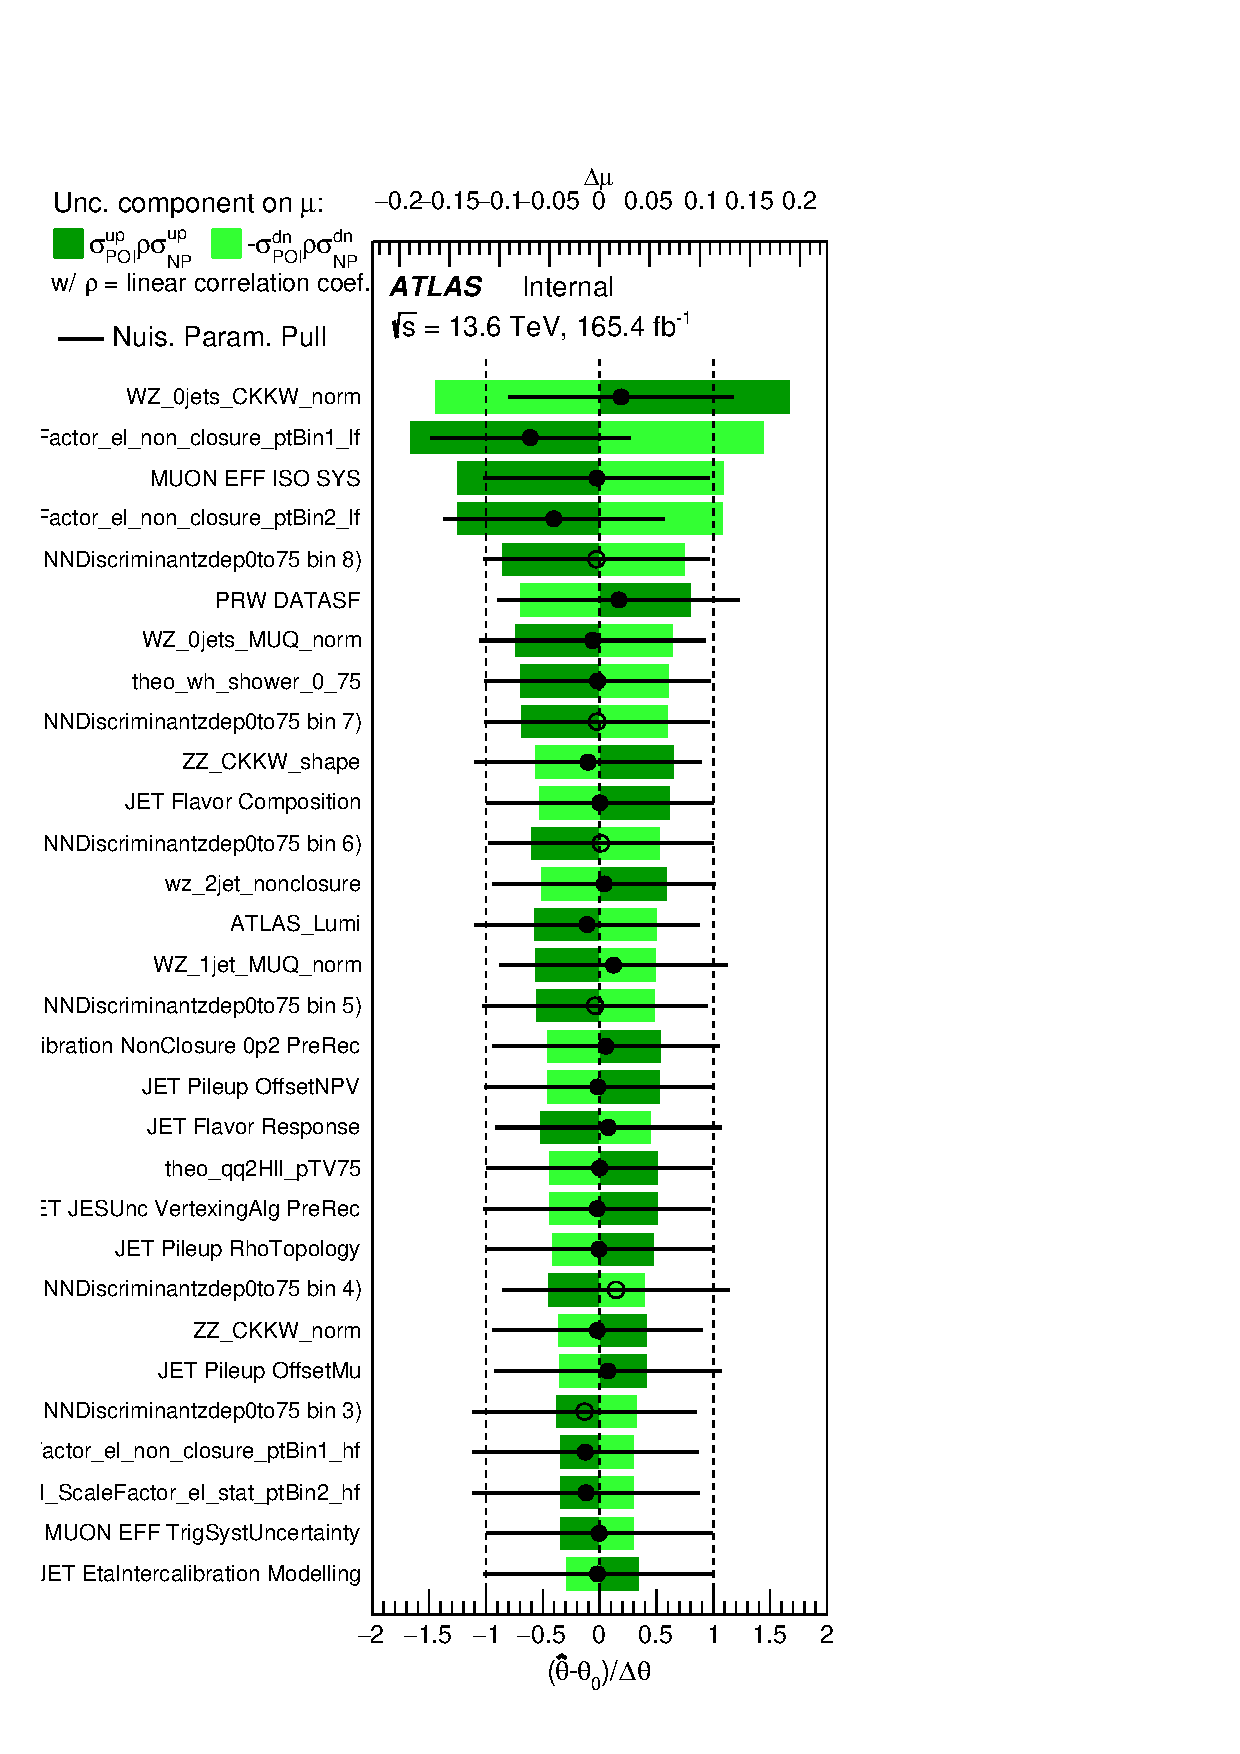
\includegraphics[width=0.3\linewidth]{figures/appendix/wh_stxs_results/rankings/Ranking_mu_WH_0_75_Breakdown_zdep_stxs.pdf}
    }
    \subfloat[Ranking: $75 < \ptv{} < 150$~GeV.]{
        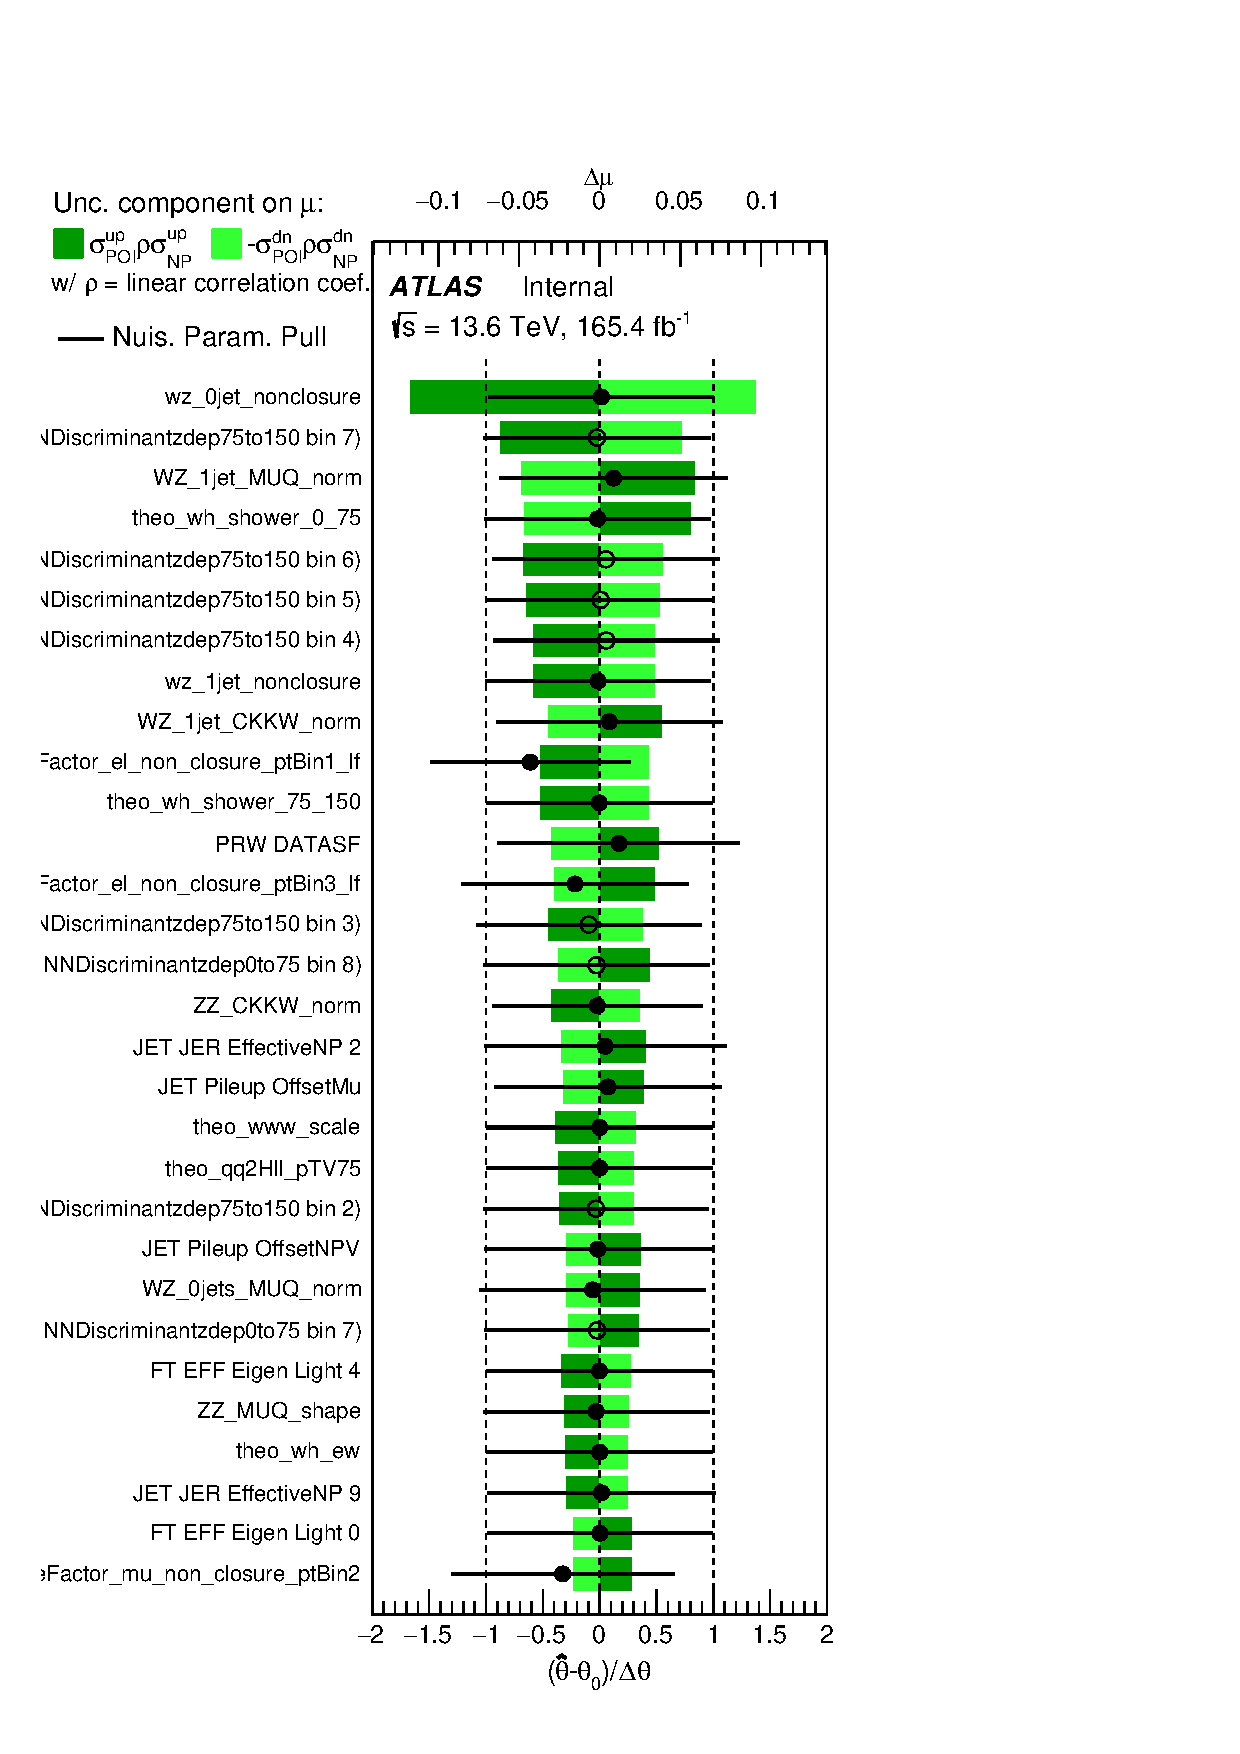
\includegraphics[width=0.3\linewidth]{figures/appendix/wh_stxs_results/rankings/Ranking_mu_WH_75_150_Breakdown_zdep_stxs.pdf}
    }
    \subfloat[Ranking: $\ptv{} > 150$~GeV.]{
        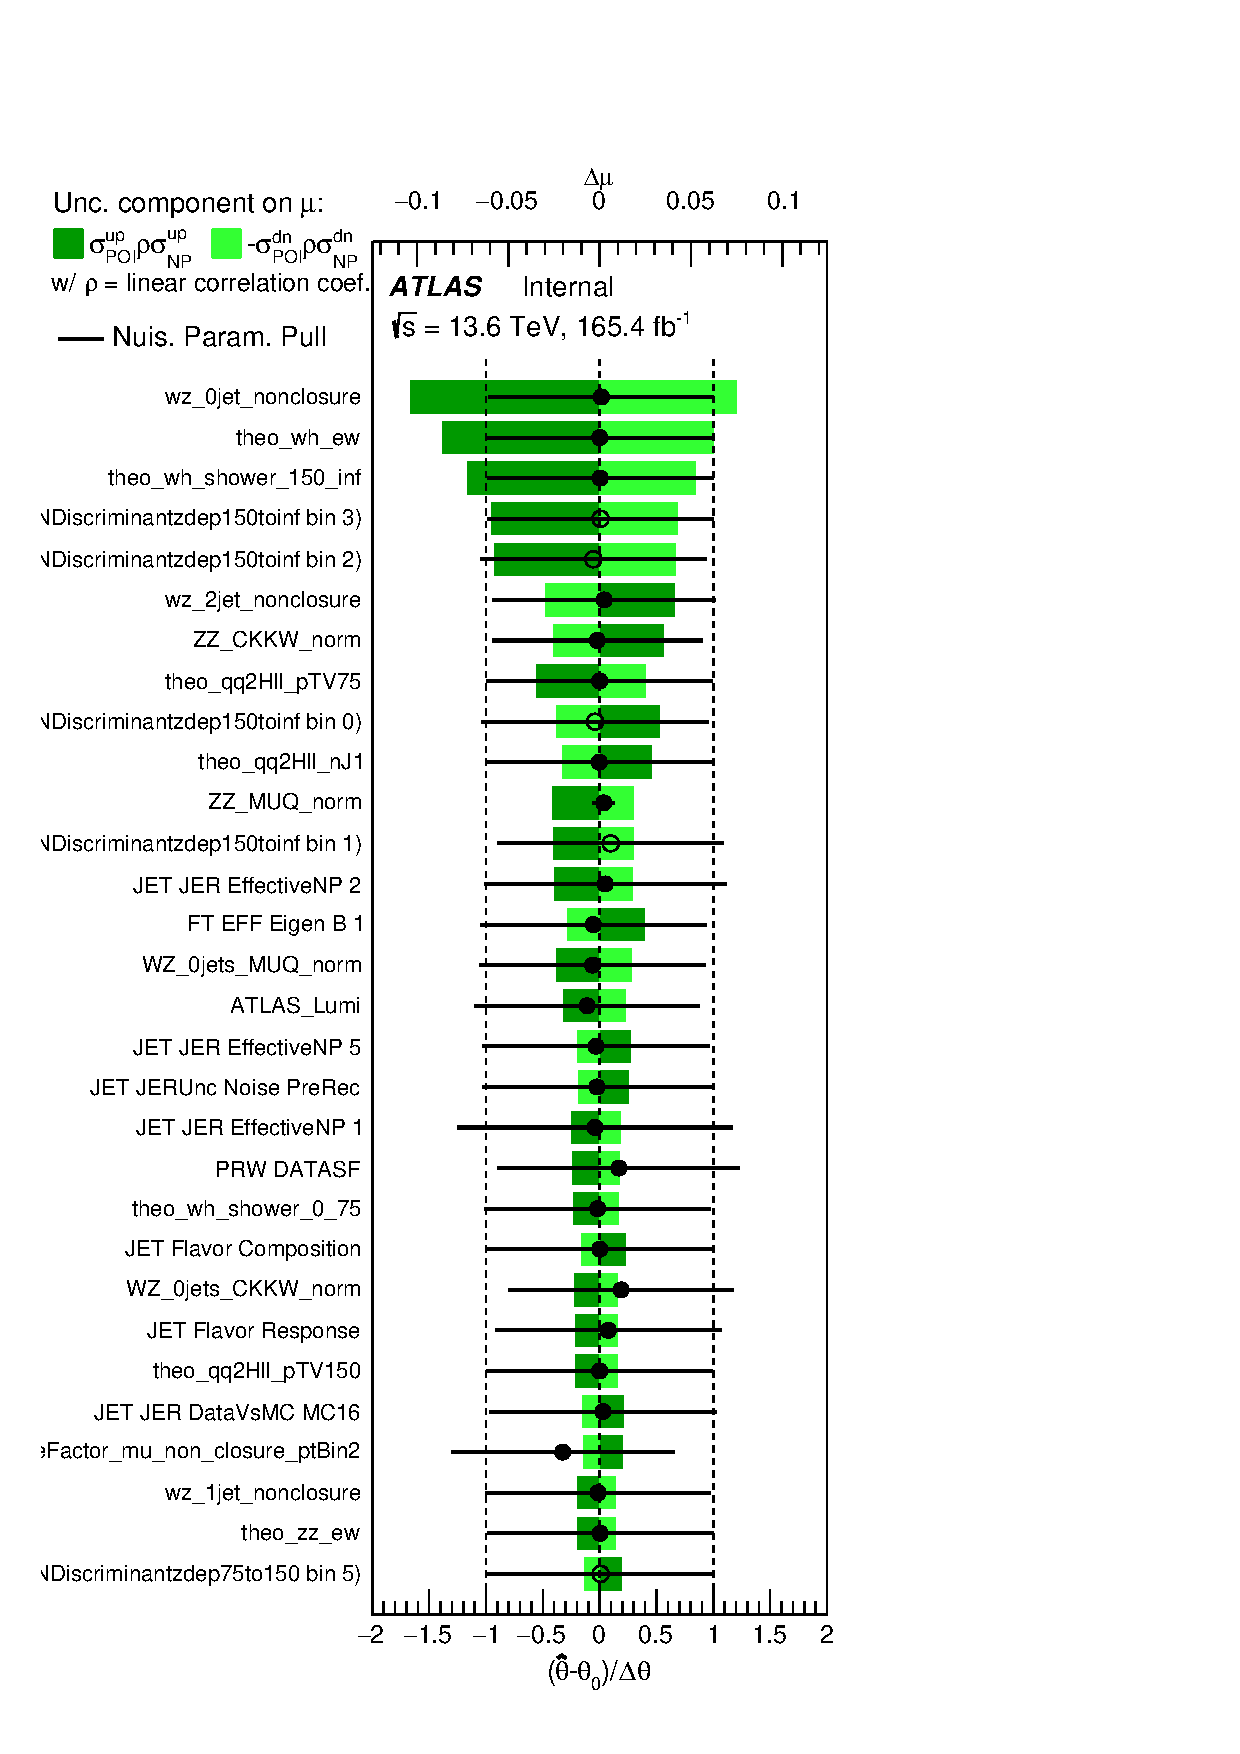
\includegraphics[width=0.3\linewidth]{figures/appendix/wh_stxs_results/rankings/Ranking_mu_WH_150_inf_Breakdown_zdep_stxs.pdf}
    }
    \caption{Systematic ranking plots for the \zdep{} \wh{} STXS signal regions: (a) $0 < \ptv{} < 75$~GeV, (b) $75 < \ptv{} < 150$~GeV, and (c) $\ptv{} > 150$~GeV.}\label{fig:wh_stxs_ranking_plots_zdep}
\end{figure}

\begin{figure}[htp]
    \centering
    \subfloat[Ranking: $0 < \ptv{} < 75$~GeV.]{
        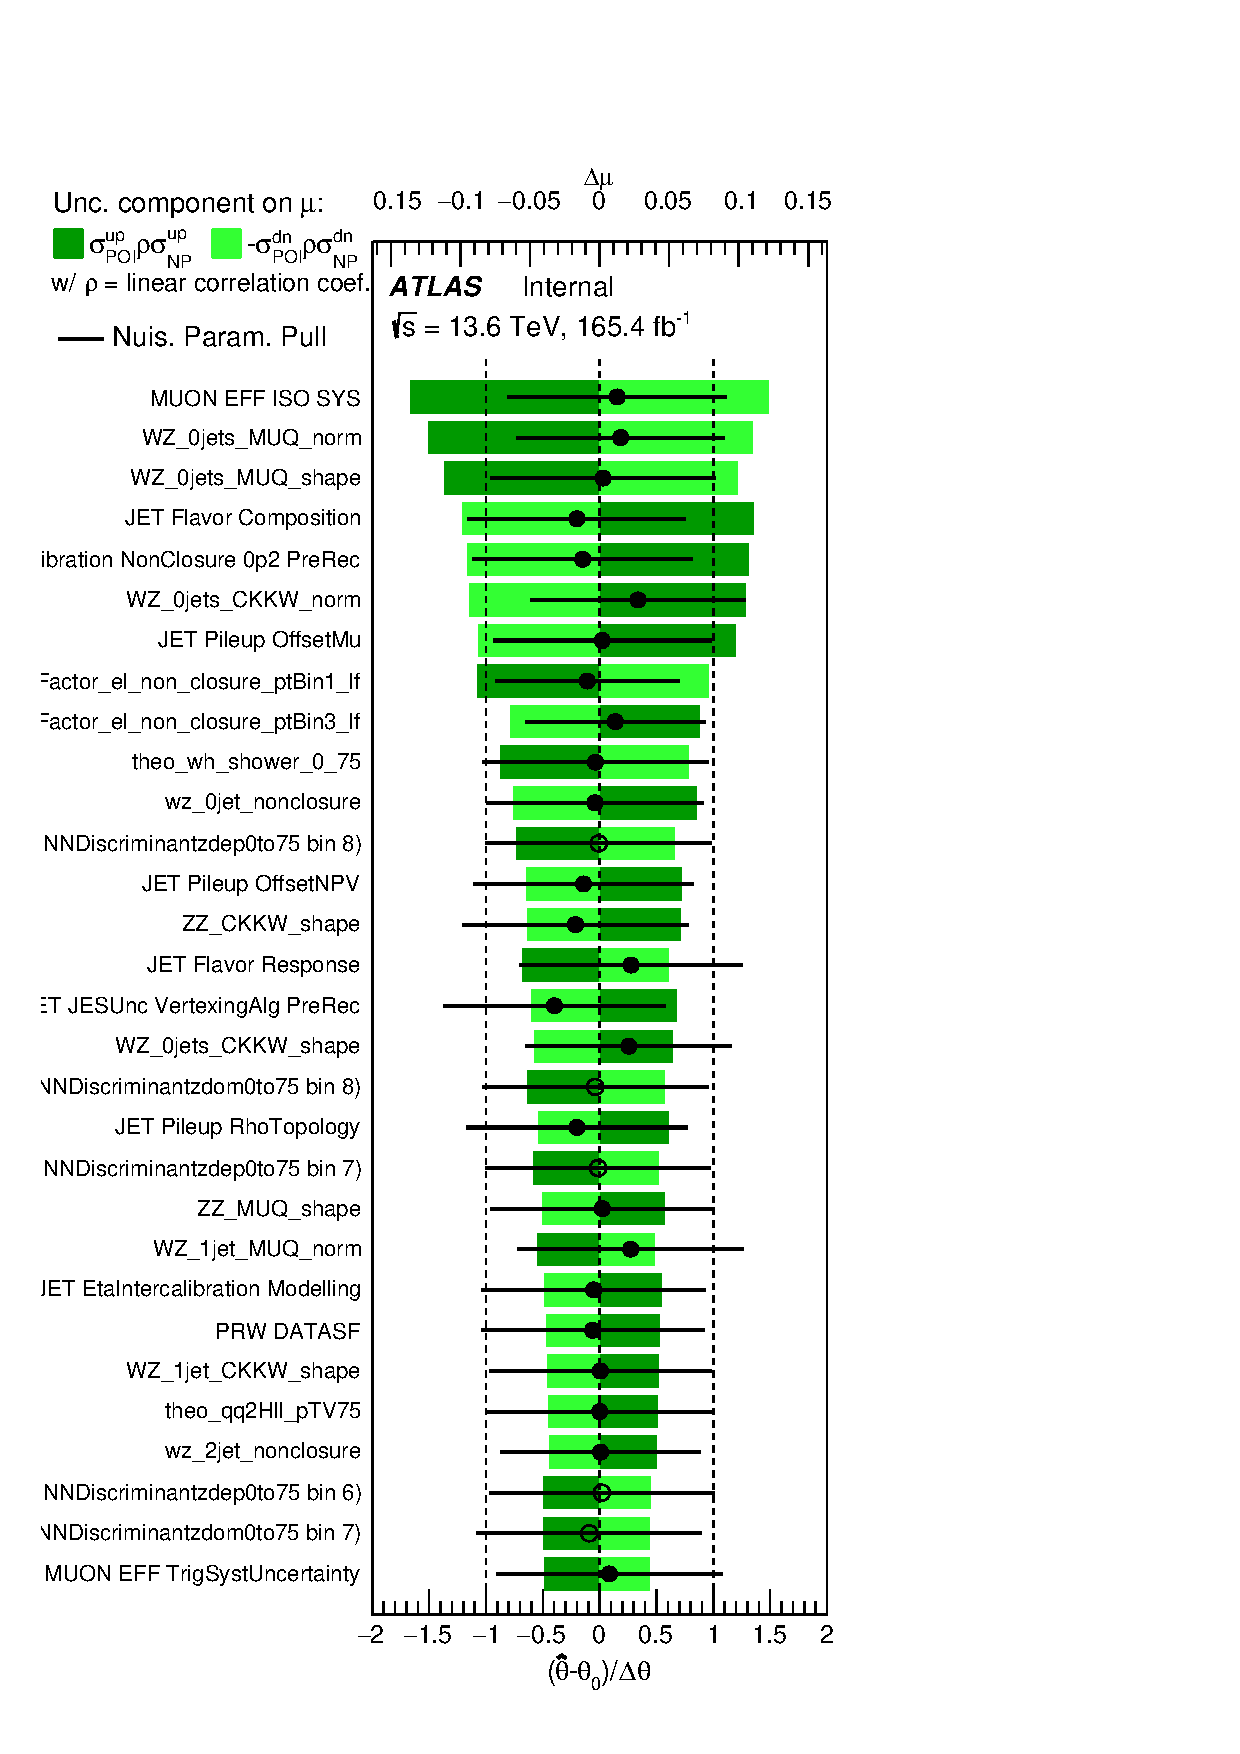
\includegraphics[width=0.3\linewidth]{figures/appendix/wh_stxs_results/rankings/Ranking_mu_WH_0_75_Breakdown_combined_stxs.pdf}
    }
    \subfloat[Ranking: $75 < \ptv{} < 150$~GeV.]{
        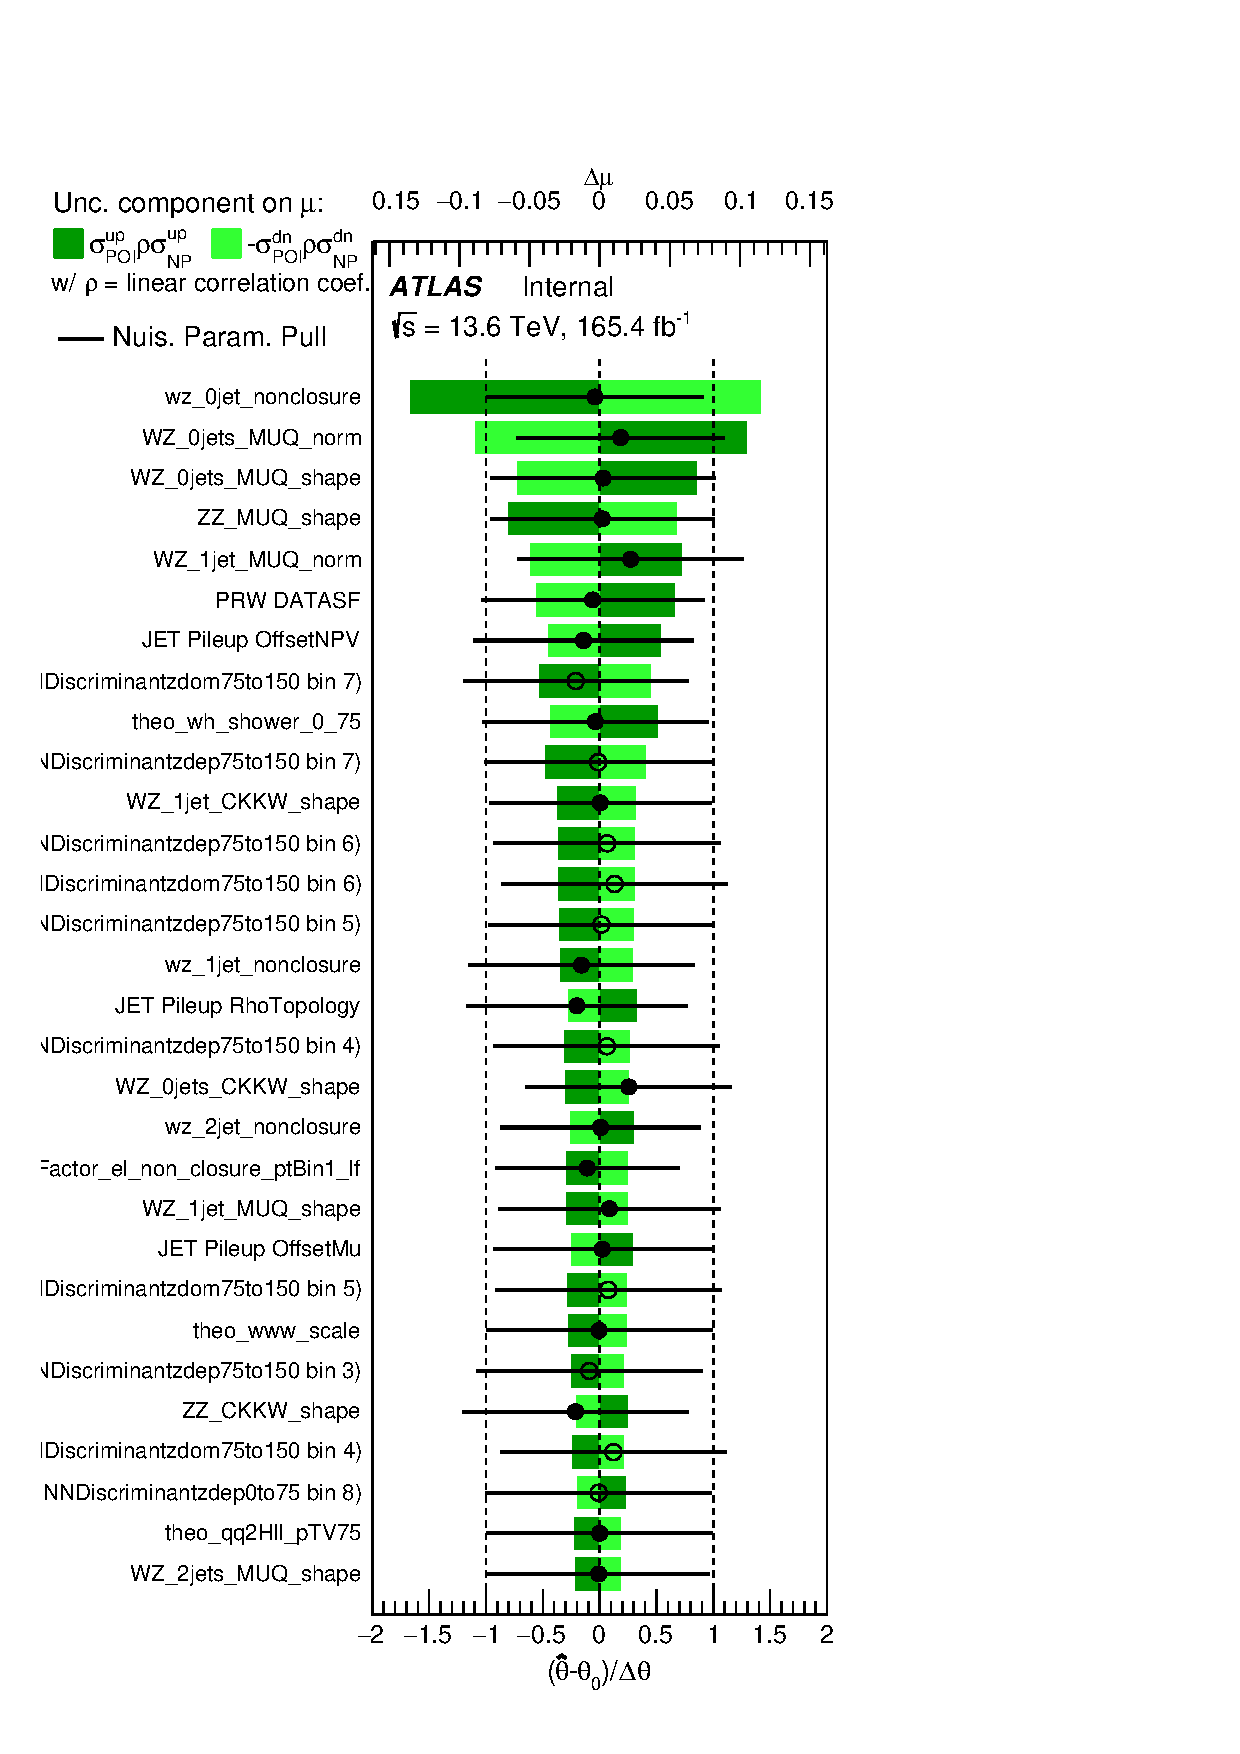
\includegraphics[width=0.3\linewidth]{figures/appendix/wh_stxs_results/rankings/Ranking_mu_WH_75_150_Breakdown_combined_stxs.pdf}
    }
    \subfloat[Ranking: $\ptv{} > 150$~GeV.]{
        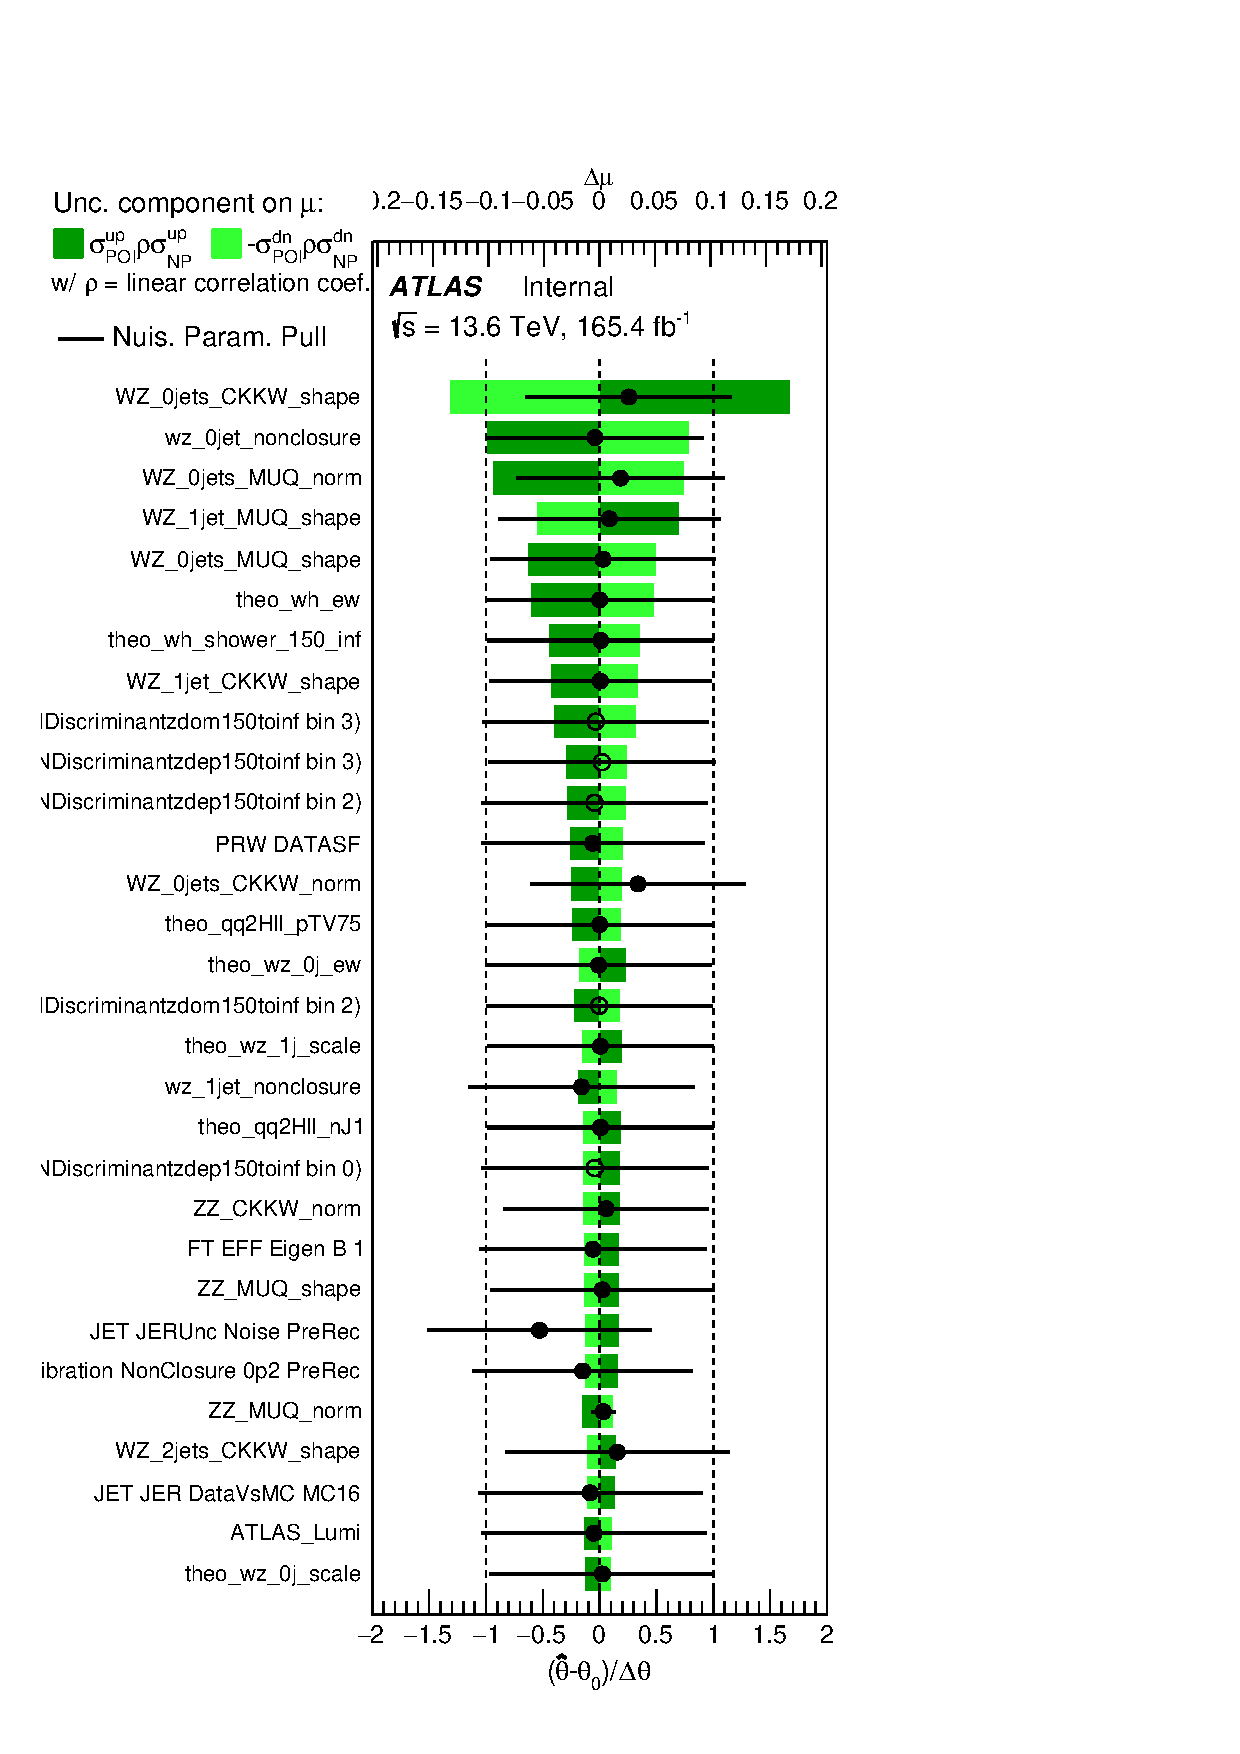
\includegraphics[width=0.3\linewidth]{figures/appendix/wh_stxs_results/rankings/Ranking_mu_WH_150_inf_Breakdown_combined_stxs.pdf}
    }
    \caption{Systematic ranking plots for the combined \wh{} STXS signal regions: (a) $0 < \ptv{} < 75$~GeV, (b) $75 < \ptv{} < 150$~GeV, and (c) $\ptv{} > 150$~GeV.}\label{fig:wh_stxs_ranking_plots_combined}
\end{figure}
\clearpage{}